\section{Results}

\subsection{Precursor Results}
After 12000 seconds of simulation time, the ABL precursor simulation showed fully developed atmospheric boundary layers.  The temperature profile of the precursor ABL simulation shows the capping inversion that limits boundary layer growth and vertical motion above 750 m.  Figures~\ref{fig:neutralABLPrecursorVelocity}  show the fully developed flow fields for neutral and unstable ABL's after they've been allowed to spin up for 12000 seconds.  

%% neutralABLPrecursorVelocity %%
\begin{figure}
\centering
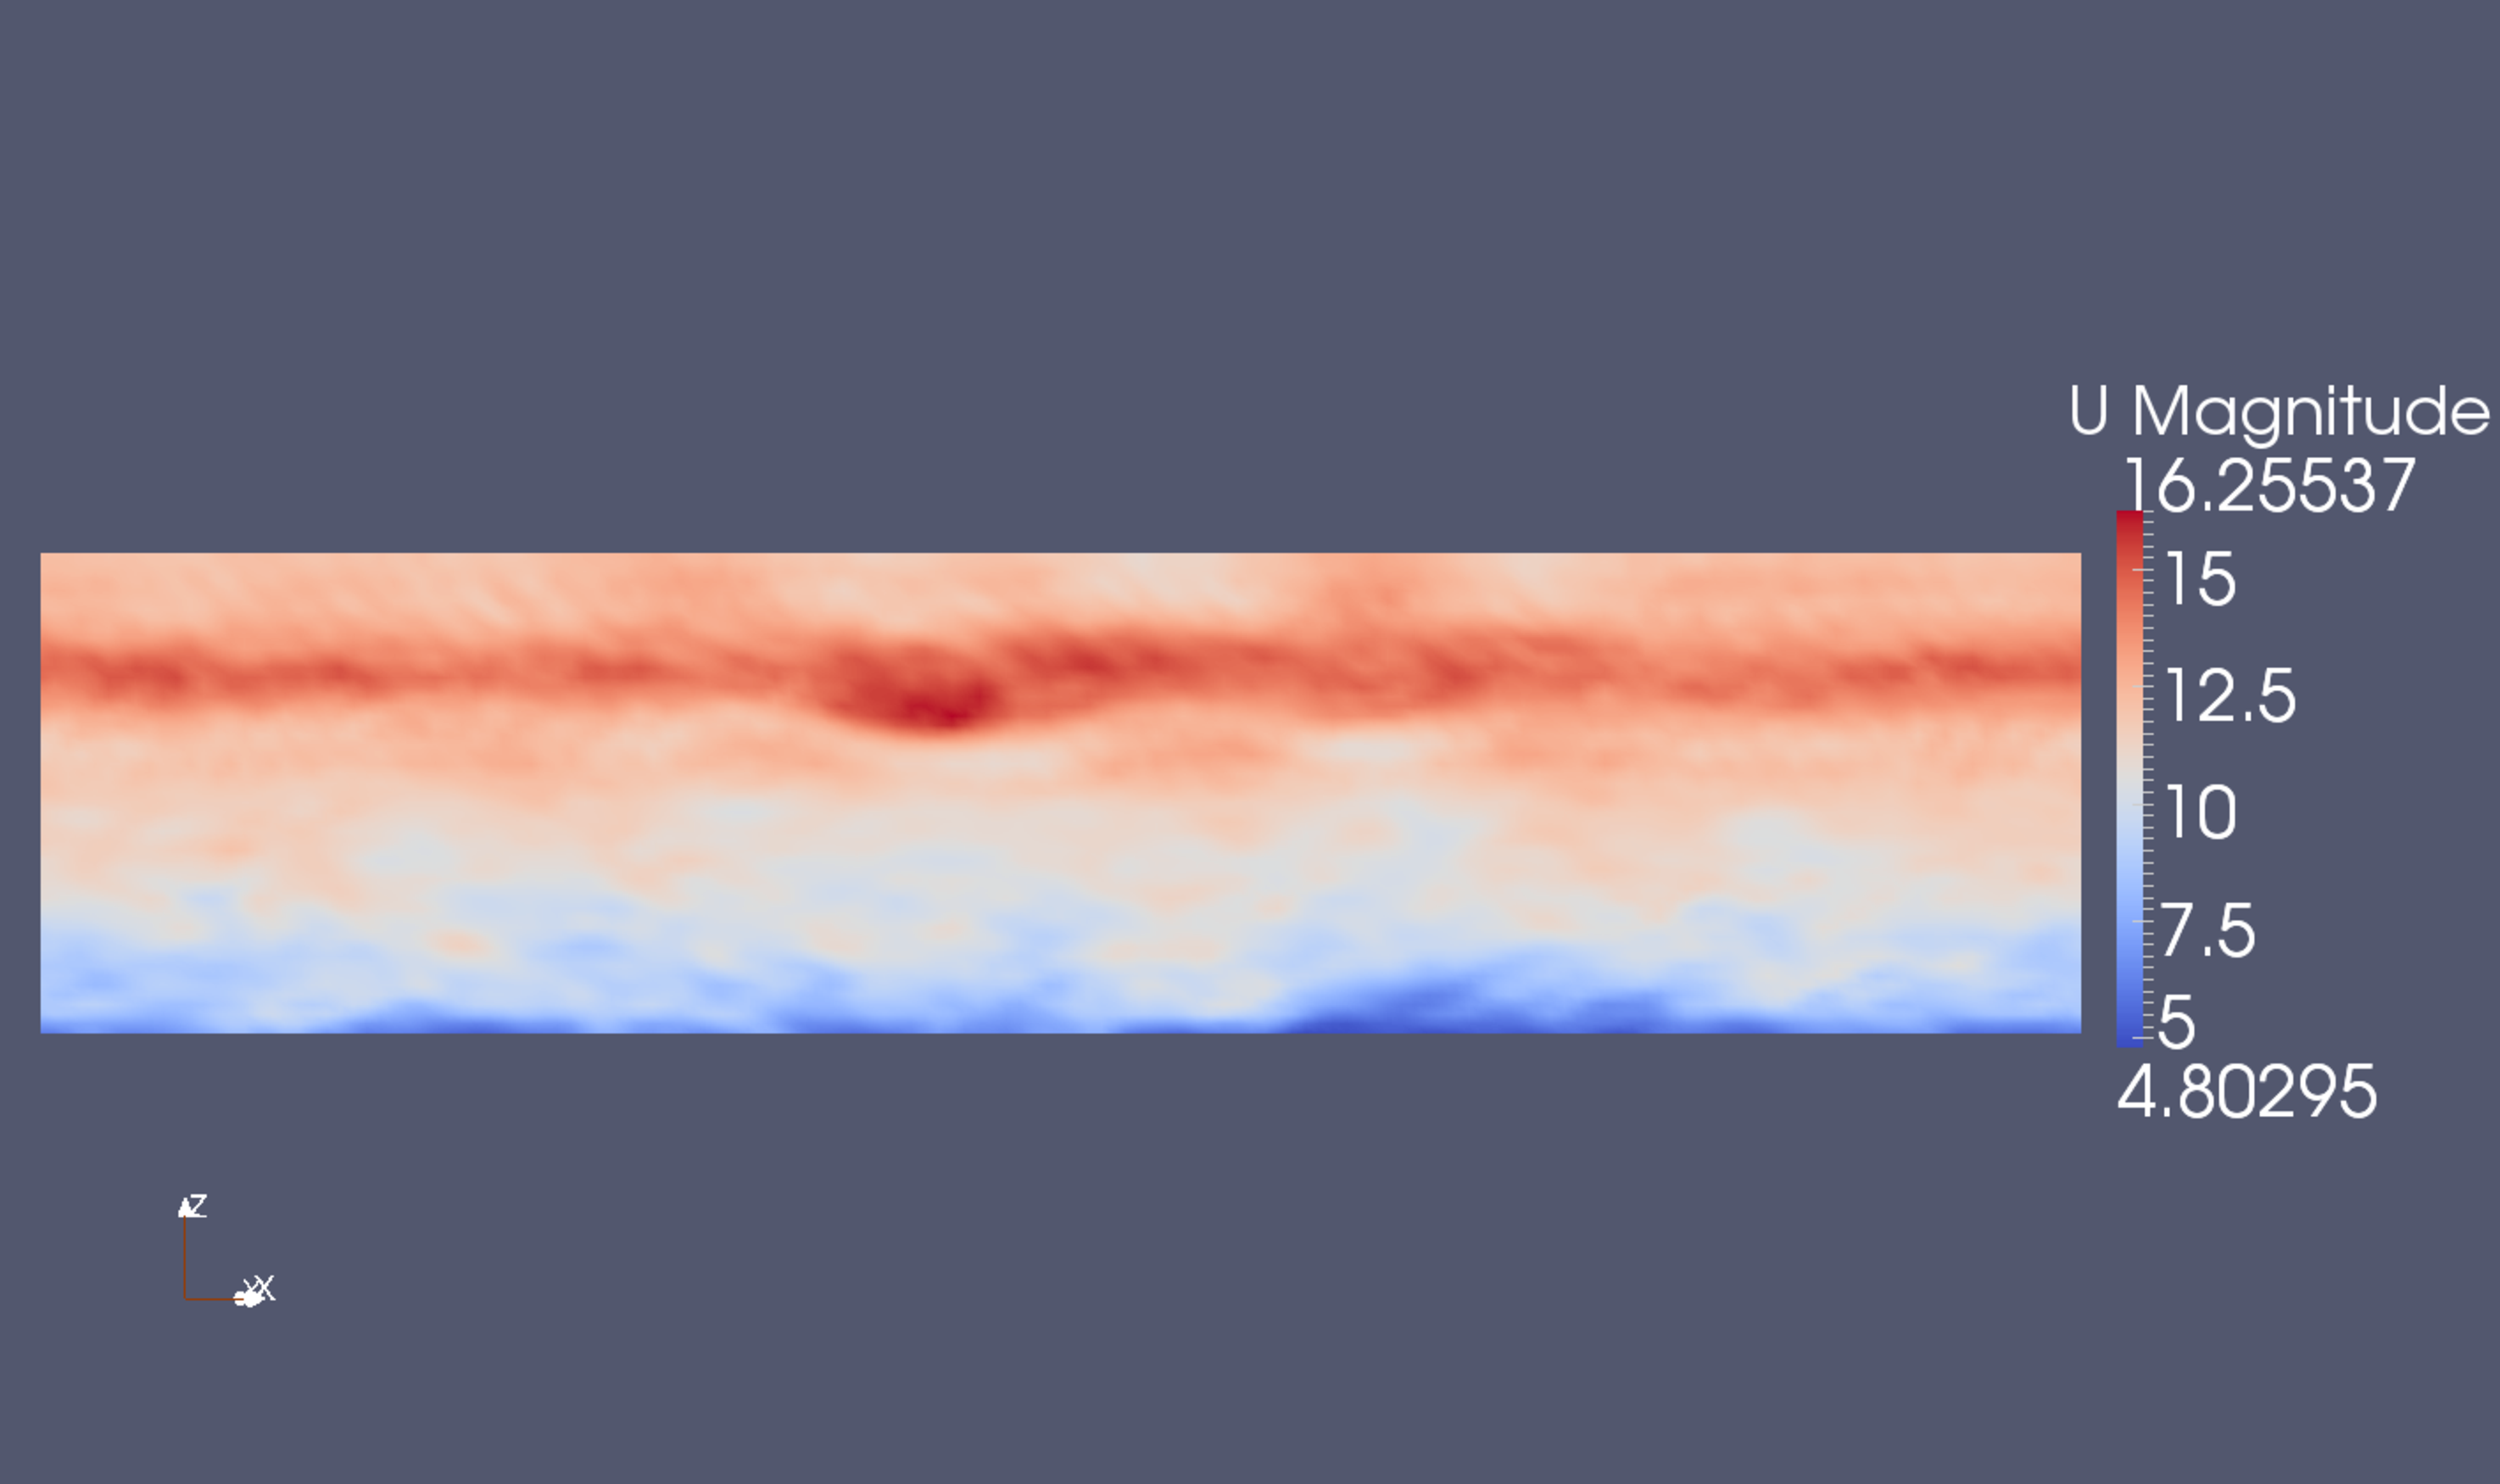
\includegraphics[width=\textwidth]{images/neutralABLPrecursorVelocity}
\caption{Precursor flow for the neutral ABL case}
\label{fig:neutralABLPrecursorVelocity}
\end{figure}

The OBL Precursor was run to 6000 seconds, which represents seven large-eddy turnovers \cite{churchfield_large-eddy_2012}. At this point, the pressure gradient drove our velocity at 35 meters to 1.9 m/s and 2.2 m/s. The vertical velocity profile for the flow is shown in Figure~\ref{fig:ocean-vertical-speed-profile}.

%% ocean-vertical-speed-profile %%
\begin{figure}
\centering
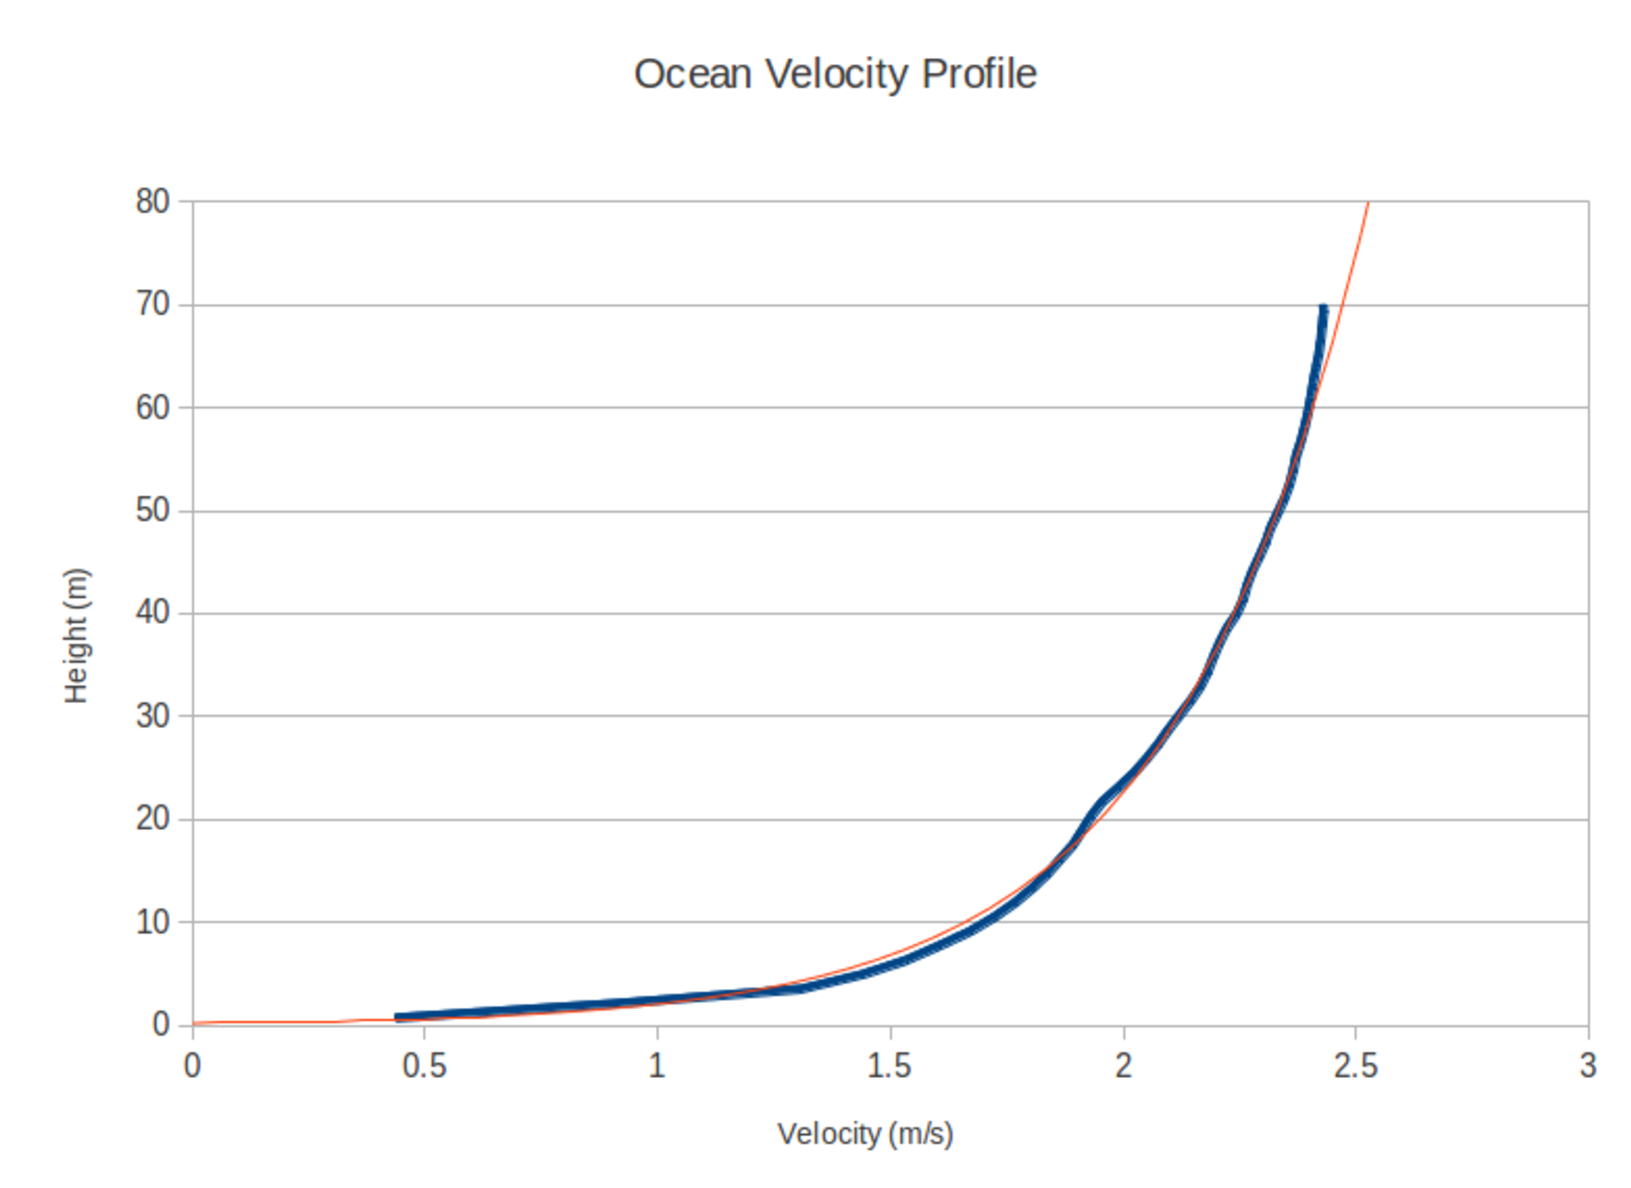
\includegraphics[width=.6\textwidth]{images/ocean-vertical-speed-profile}
\caption{Vertical velocity profile for the OBL}
\label{fig:ocean-vertical-speed-profile}
\end{figure}

The precursor simulations show realistic coherent turbulent structures that are crucial in generating realistic load distributions.  The different stability cases also exhibit realistic vertical mixing and shear profiles, with the unstable case showing a better mixed boundary layer.

\subsection{Actuator Line Results}
After fully developing the atmospheric boundary layer in the absence of wind turbines, we insert a single actuator line turbine and run the simulation for another 250 seconds.  The results lead to several interesting insights.  First, there is nontrivial flow leakage at the root of the blades that persists for about two rotor diameters downstream.  This region where the blade airfoil properties are still discernible is the "near-wake" region\cite{sanderse_review_2011}.  Further downstream in the "far-wake" region the blade-specific effects have diffused into an amorphous wake, but the velocity deficit that is characteristic of the far-wake is present for eight to ten rotor diameters.  Figures XX show average velocity profiles and Figures XX show instantaneous velocity profiles at 250 seconds.  The instantaneous velocities also show horizontal and vertical meandering of the wake that is likely caused by instabilities in the boundary layer.

\subsubsection{Numerical Artifacts}
Interestingly, we also observe numerical artifacts in the CFD results located at the transition between grid refinement regions.  Figure~\ref{fig:neutralWindPlantAvgVelPlanMeshRefine} shows the average velocity at hub height for the unstable ABL with the actual grid cells overlaid on the flow field.  Clearly, the artifacts are generated at the abrupt transition between adjacent refinement levels.   Confirming these results, the ocean turbine simulation, where the grid refinement was constant across the entire domain, did not show any signs of artifacts -- this is shown in Figure~\ref{fig:OceanMeshRefinement}. However, a single grid refinement level is not the ideal solution -- conversations with the SOWFA creators, Matt Churchfield and Sang Lee, suggest that a spatial filter or mesh smoothing function could help alleviate these anomalies.

%% neutralWindPlantActuatorMeshRefinement %%
\begin{figure}
\centering
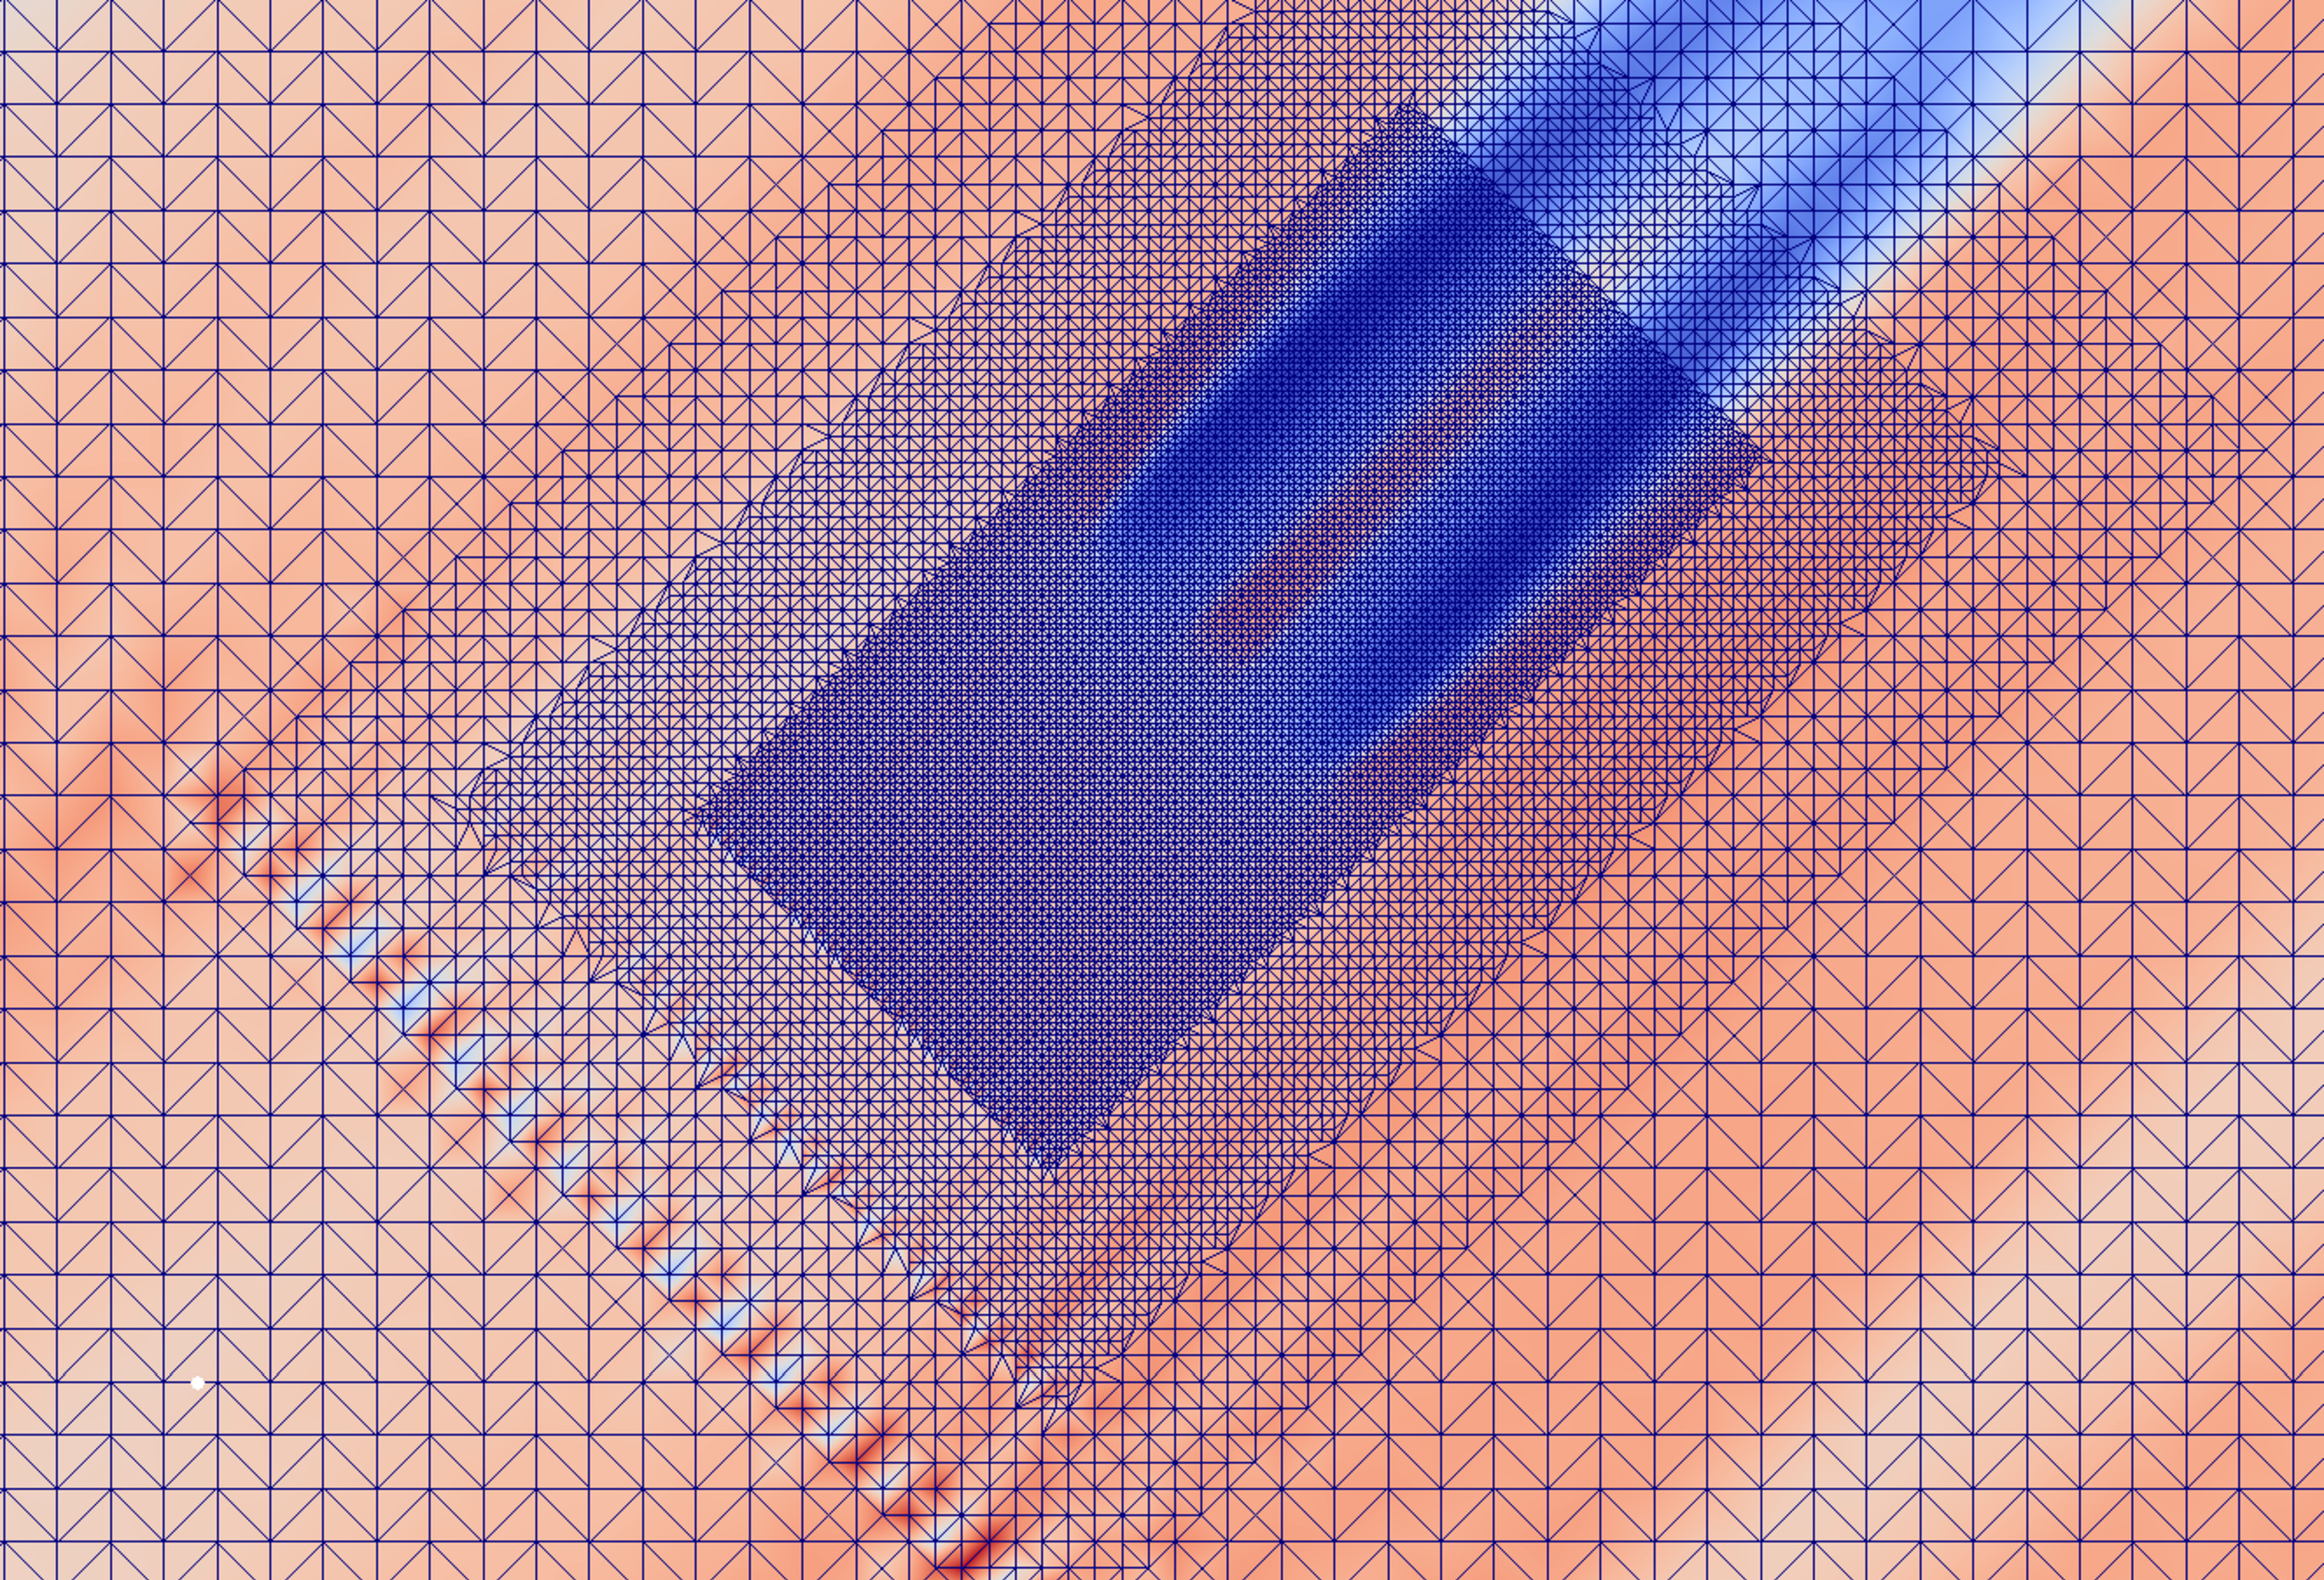
\includegraphics[width=\textwidth]{images/neutralWindPlantAvgVelPlanMeshRefine}
\caption{Numerical artifacts present in the ABL wind turbine simulation}
\label{fig:neutralWindPlantAvgVelPlanMeshRefine}
\end{figure}

%% OceanMeshRefinement %%
\begin{figure}
\centering
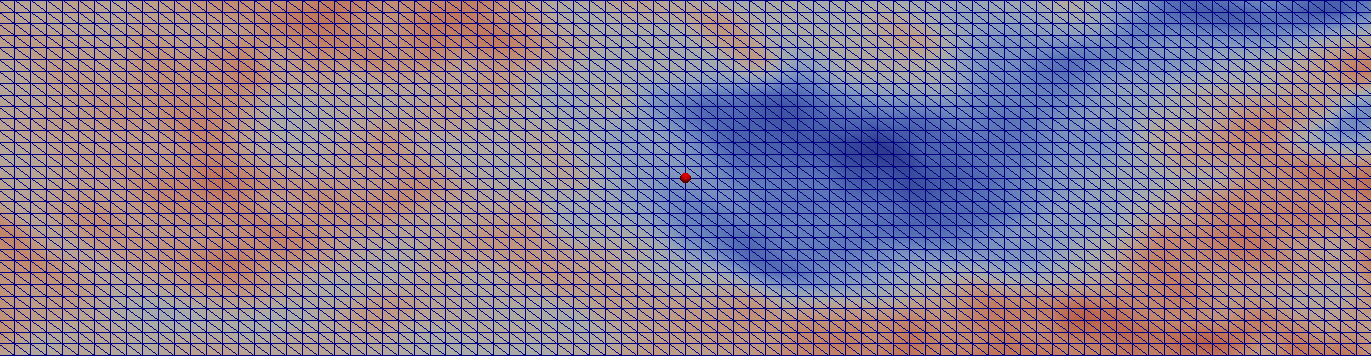
\includegraphics[width=\textwidth]{images/OceanMeshRefinement}
\caption{Ocean wind turbine simulation without artifacts}
\label{fig:OceanMeshRefinement}
\end{figure}



\subsubsection{Vertical wake oscillation}

One very notable feature of the ocean current turbine flow was the extent to which vertical flow oscillation dominated the velocity profile. Figure~\ref{fig:ocean-side-profile} shows the movement of the vertical oscillation, with three snapshots from 100, 200 and 300 seconds. While vertical oscillations were certainly noted in the wind energy simulation, the extent of the ocean turbine oscillatiosn is comparatively much greater, with the peaks of the oscillation covering most all of the 70 meter vertical domain.

%% ocean-side-profile1 %%
\begin{figure}
\centering
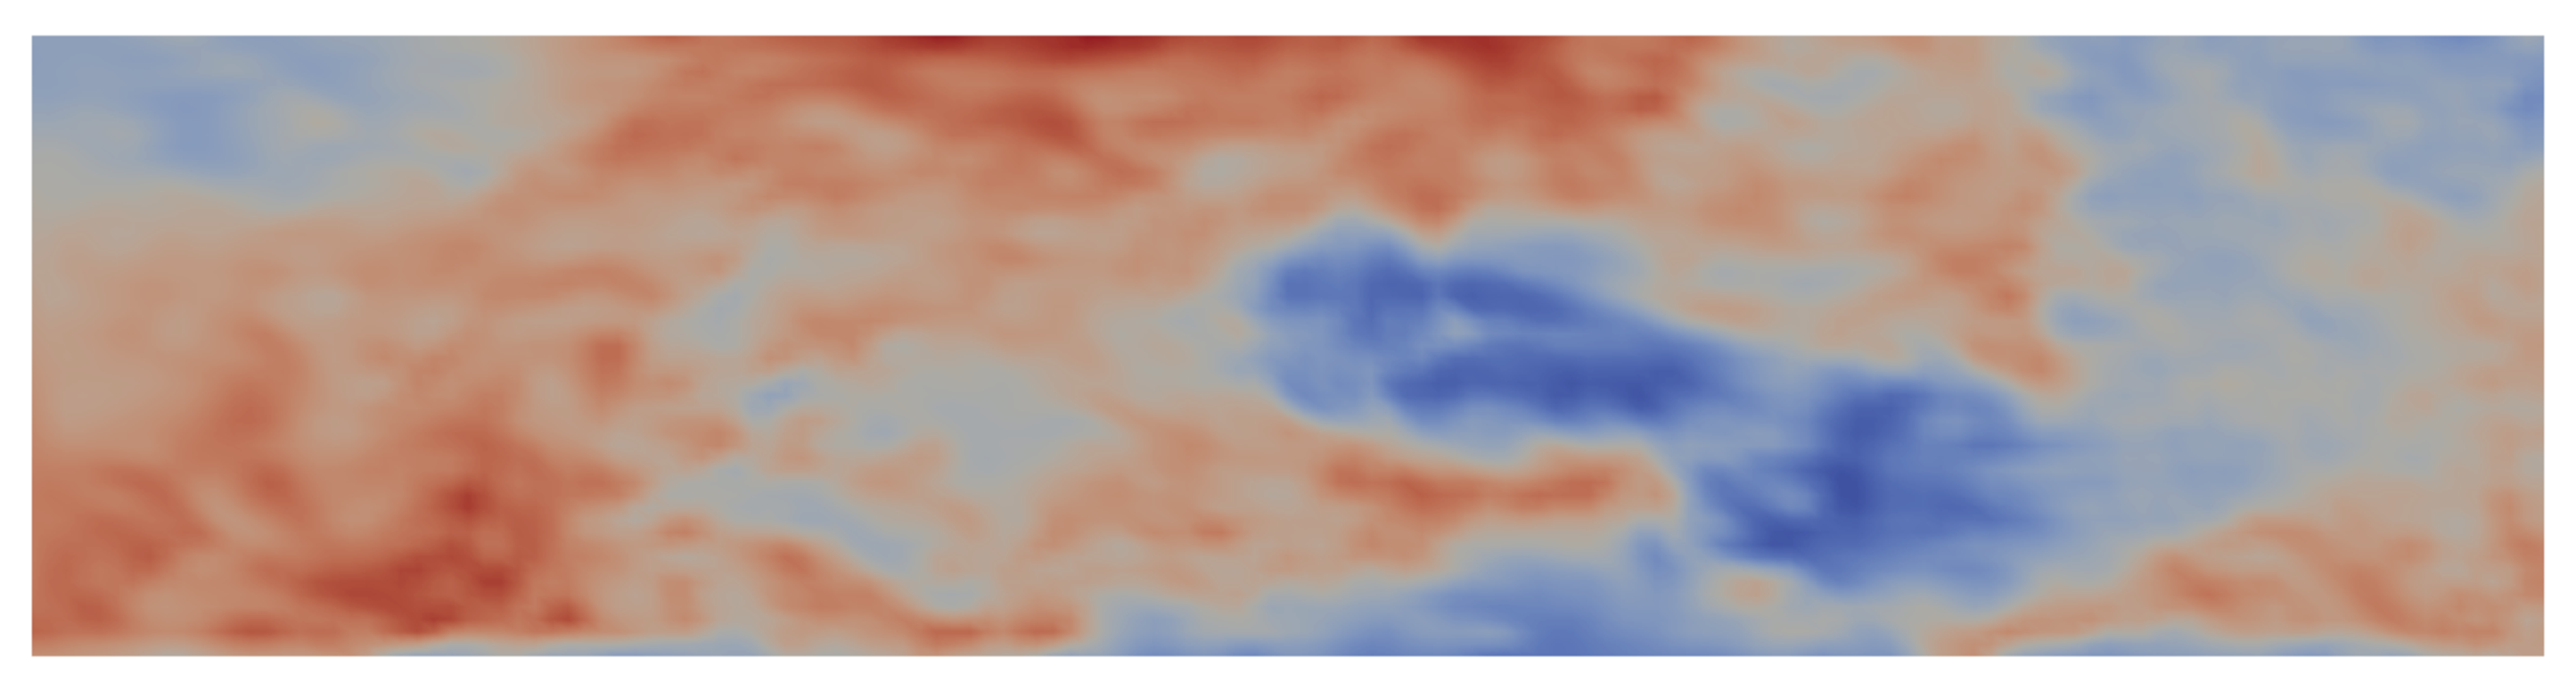
\includegraphics[width=\textwidth]{images/ocean-side-profile1}
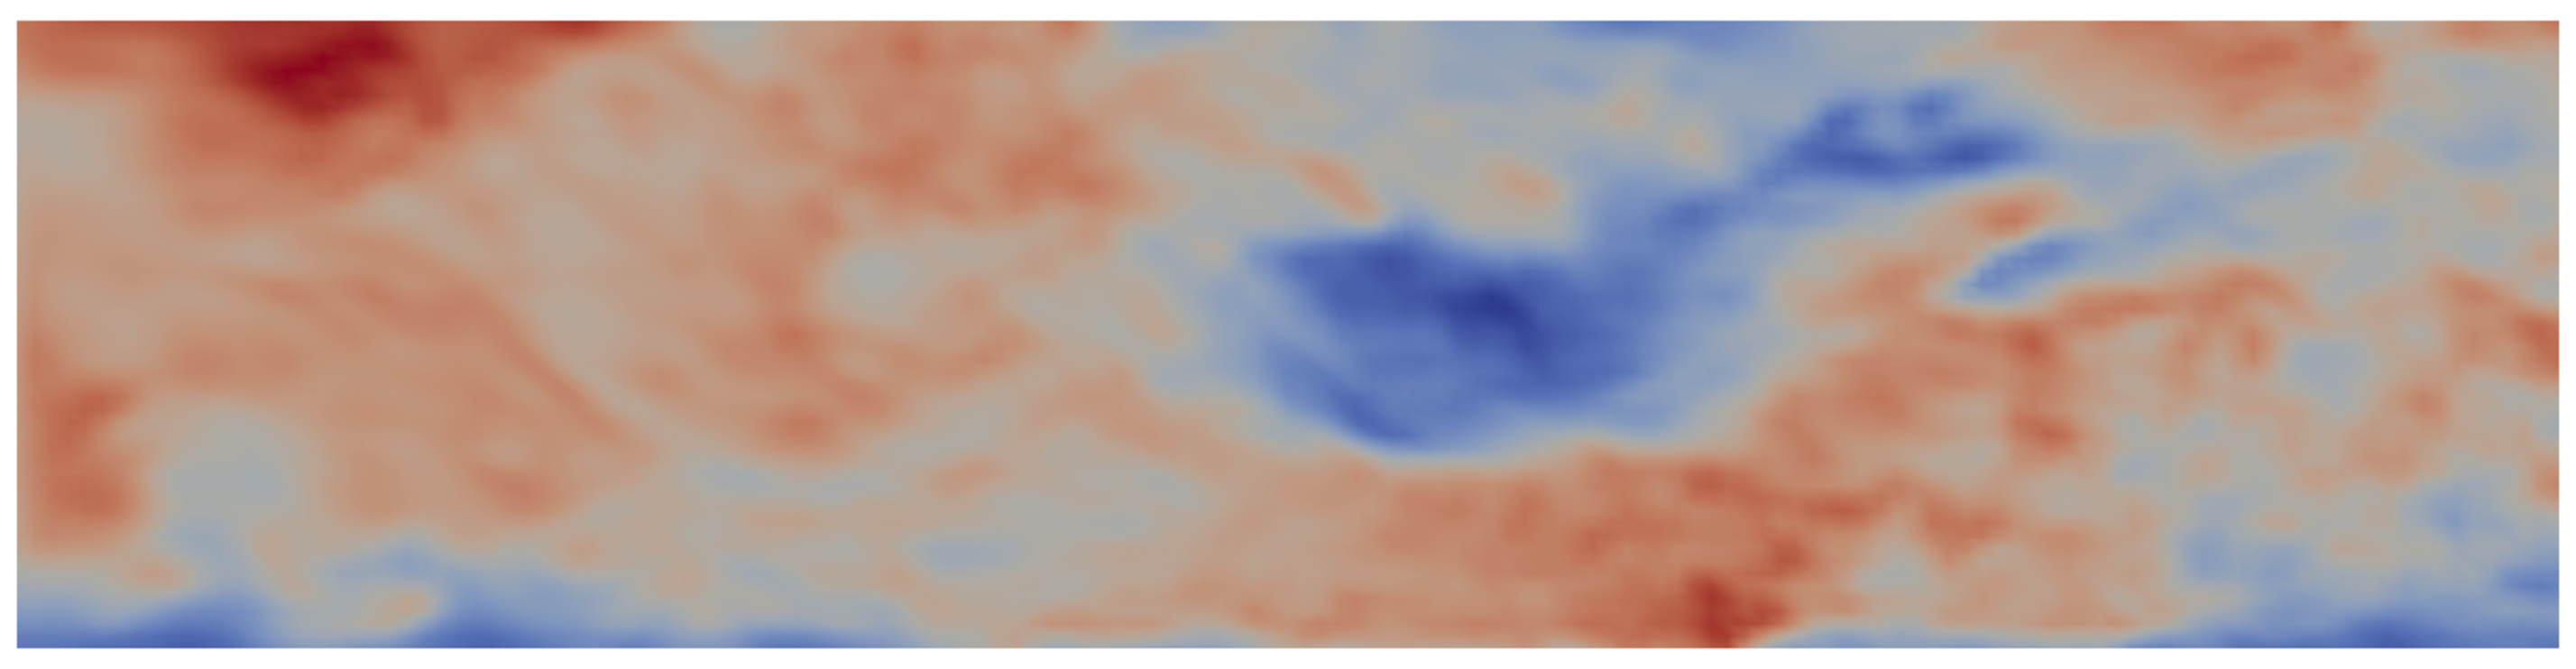
\includegraphics[width=\textwidth]{images/ocean-side-profile2}
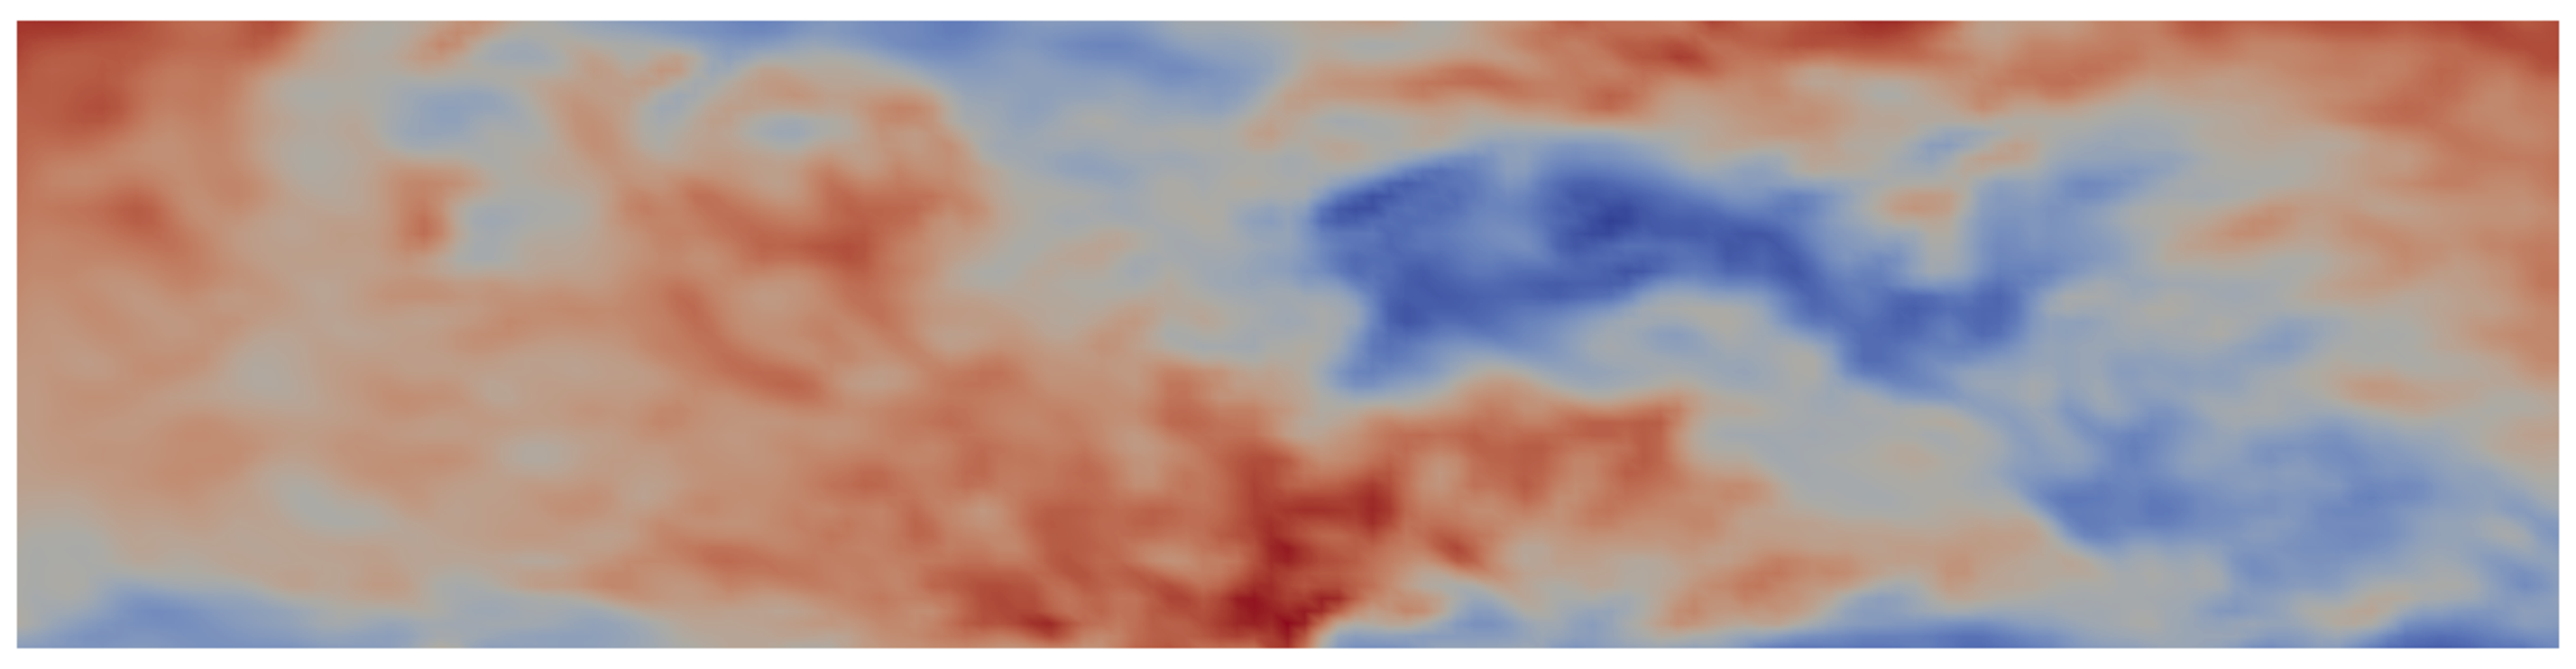
\includegraphics[width=\textwidth]{images/ocean-side-profile3}
\caption{Ocean turbine flow snapshots at t = 100s, 200s and 300s}
\label{fig:ocean-side-profile}
\end{figure}
